\documentclass[11pt,twoside]{article}
\usepackage[spanish, es-tabla]{babel}
\usepackage[utf8]{inputenc}
\usepackage{booktabs}
\usepackage{booktabs}     % tablas 
\usepackage{tabulary}     % tablas
\usepackage{graphicx}      % poner imagenes 
\usepackage{float}         % para fijar las imagenes con h y H
\usepackage{fancyhdr}

% para insertar codigo R

% Margins
\topmargin 0.02cm
\headheight 0.02cm
\textwidth 15.50cm
\oddsidemargin .0in
\evensidemargin .0in

\date{}

\begin{document}


	
\fancypagestyle{firststyle}
{
	\fancyhead[R]{ \tiny{Facultad de Ciencias, Facultad de Minas \\
			Universidad Nacional de Colombia, Sede Medellín\\
			2019}}
	\fancyhead[L]{}
	\fancyfoot[LO,RE]{}
	\fancyfoot[LE,RO]{ \vspace{10pt}\thepage}
	\renewcommand{\headrulewidth}{0pt}
	\renewcommand{\footrulewidth}{0pt}
}

\thispagestyle{firststyle}
\begin{center}
	\Large{{\bf STATISOFT 2.0\\
			\vspace{20pt}  PREDICCIÓN DEL NIVEL DE SATISFACCIÓN DE LAS MADRES SOLTERAS EN COLOMBIA\\ 
			\vspace{10pt}}}
\end{center}

{\normalsize{
		Heber Esteban Bermúdez			\footnote{\footnotesize{ hebermudezg@unal.edu.co}}
		John Bryan Yepez				\footnote{\footnotesize{ jbyepezh@unal.edu.co}},
		Simon Zapata 					\footnote{\footnotesize{sizapatagu@unal.edu.co}},
		Nelson Ordónez 			\footnote{\footnotesize{neordoñezm@unal.edu.co}}
}}




\begin{abstract}
\noindent
Es importante para muchas organizaciones, entidades, fundaciones y en especial programas del gobierno nacional saber sobre la calidad de vida y el nivel de satisfacción de los colombianos, el presente trabajo está enfocado en analizar el nivel de satisfacción de las madres solteras en Colombia, y analizarlo con un conjunto de variables particulares asociadas a la estructura del hogar y el acceso a tecnologías de la información y comunicación entre otras, es por eso, que el presente proyecto pretende conocer cuáles son esos factores que más afectan el nivel de satisfacción las madres solteras en Colombia como también crear una aplicación web para predecir este nivel de satisfacción. Para conocer este fenómeno el grupo de trabajo \textbf{Statisoft 2.0} empleo datos abiertos del Departamento Administrativo Nacional de Estadística \textbf{(DANE)} de la Encuesta de Calidad de Vida del año 2017 y usando técnicas estadísticas con los software \textbf{R} y el paquete Shinny crea un modelo estadístico y una aplicación de uso público que logra predecir el cómo se comporta la satisfacción de las madres solteras usando las algunas de las variables de la encuesta, es por eso que el grupo \textbf{StatiSoft 2.0} crea un entendimiento a partir de los conceptos amplios como calidad de vida y madre soltera para desenlazar con el desarrollo de la aplicación. \\
\textbf{Palabras Clave}: satisfacción personal, calidad de vida, madre soltera.
\end{abstract}



%***-------------------------------------INTRODCUCCION-----------------------------------------------------
\section{Introducción}
\noindent
La calidad de vida es un concepto de amplio bagaje que se ha tratado desde hace un tiempo en Colombia debido a la estratificación socio-económica. La calidad de vida hace alusión a cinco áreas distintas como lo son: Bienestar físico, bienestar material, bienestar social, desarrollo y bienestar emocional; siendo este último uno de los factores psicológicos mas importantes para la satisfacción con la calidad de vida y el desarrollo de las otras cuatro áreas. La satisfacción con la vida busca e intenta definir  que es una buena vida y evaluar lo bien que vivimos, aunque aún así siga siendo un juicio subjetivo, cada persona está supeditada a encontrar su punto de equilibrio para decir que tan satisfecha está con su vida.
\\
\\
\noindent
El nivel de satisfacción es una apreciación subjetiva que aporta al bienestar general, ya que permite evaluar de manera personal cómo va tu vida en relación a lo que esperas de ella; por eso esta definición juega un papel muy importante en los hogares colombianos. Según el diario El Heraldo, para el 2017 había 22 millones de mujeres en el país, de las cuales sólo el 41,9{\%} tienen una ocupación formal o informal fuera del hogar y según datos del DANE, el 56{\%} de esas 22 millones de mujeres son cabeza de familia, es decir, madres solteras. Por lo anterior, se evidenca diferencia marcada tanto de madres solteras como de la crítica desventaja en términos laborales entre hombres y mujeres.
\\
\\
\noindent
Con el objetivo de mostrar el nivel de satisfacción de las madres solteras en Colombia, la Encuesta de Calidad de Vida del 2017 publicada por el DANE es la materia prima principal para responder la pregunta planteada: ¿Qué afecta la satisfacción de las madres solteras? Además, a la persona interesada le permite saber cuál es el nivel de satisfacción de la madre soltera según los esquemas de preguntas formulados por el DANE, los cuales en el presente trabajo son tratados como variables. Dicha Encuesta de Calidad de Vida fue formulada a través de un diseño muestral probabilístico, estratificado, multietpico, de conglomerados.
\\
\\
\noindent
Ante esta duda de cuál es el nivel de satisfacción de las madres solteras y qué factores influyen, es creada la aplicación \textbf{StatiSoft 2.0}, la cual tiene un desarrollo que podrá predecir el nivel de satisfacción de las madres solteras en función de variables como la percepción de satisfacción en cuanto al ingreso económico, salud, seguridad, felicidad, tranquilidad, número de hijos, número de nietos, acceso a internet y uso de redes sociales, para así predecir su nivel de satisfacción.
\\
\\
Esta aplicación es de  uso abierto y  baja complejidad por lo que a empresas y personas particulares  se les facilitará usarlo, ademas de ser fundamental para promover la investigación sobre las condiciones de vida y la medición de la pobreza en los hogares colombianos, donde las poblaciones más afectadas son las madres solteras que no cuentan con ayuda para la crianza de sus hijos y el manejo del hogar.




%***------------------------------------------DEFINICIONES-----------------------------------------------
\section{Definiciones}
\noindent
A continuación se definen claramente los conceptos tratados en nuestro estudio y desarrollo del trabajo \\
\\
\textbf{Madre soltera} \\
Se denomina madre soltera generalmente a un tipo de familia monoparental, en la que una mujer lleva a cabo la crianza de los hijos y el manejo del hogar sin la compañía o apoyo de una pareja, por decisión propia o circunstancias de su entorno. En un sentido muy estricto se podría hablar con propiedad de núcleo familiar monoparental cuando el conjunto es formado por un progenitor (madre o padre, en este caso madre) y uno o varios hijos. Este núcleo puede constituir por sí solo una familia independiente (familia nuclear monoparental), o puede convivir con otras personas emparentadas. Por ejemplo, una madre (sin pareja) con dos hijos que convivan con sus padres constituye un núcleo monoparental en una familia extensa. Debido a esto no se excluyen el número de personas con las que viva la madre soltera.\\
En conclusión, para nuestro estudio hemos tomado la mujeres solteras o viudas de cualquier edad que tiene uno o más hijos en el hogar.\\
\\
\textbf{Nivel de satisfacción con la vida}\\
La satisfacción con la vida es una apreciación subjetiva que aporta al bienestar general, ya que permite evaluar de manera personal cómo va tu vida en relación con lo que esperas de ella. Tratar este tipo de temas resulta algo denso y complicado ya que la categorización de este requiere un análisis agudo según la satisfacción que tenga la persona con diferentes factores que pueden alterar su entorno y vida diaria.\\
Para la Organización Mundial de la Salud, ésta última refiere no sólo al estado completo de bienestar físico y mental sino también social y dado una fase tan subjetiva, el tipo de análisis comienza desde un aspecto psicológico.



%***------------------------------------------ ANALISIS-----------------------------------------------------

%\section{Análisis}

El objetivo principal del proyecto es 




%***---------------------------------------- METODOLOGIA-----------------------------------------------------

\section{Metodología}
\noindent
En la primera etapa del desarrollo del trabajo fue preciso hacer un análisis descriptivo previo, para observar el comportamiento de las posibles variables significativas para el modelo, y luego adoptar la metodología estadística a implementar para crear el modelo que permita hacer la correcta predicción del nivel de satisfacción de las madres solteras en Colombia. Para el estudio se usaron los datos de la encuesta nacional de calidad de vida del \textbf{DANE}, donde se seleccionaron las mujeres que cumplieran con las características de tener uno o más hijos y que fueran solteras o viudas esto acorde con la definición mencionada (ver sección \textbf{2. Definiciones}).
\\
Nuestro estudio se enfocó en analizar cómo las variables de características y composición del hogar y el acceso a tecnologías de información y comunicación afectan el nivel  de satisfacción de las madres solteras, se  realiza el análisis descriptivo de la base de datos (ver \textbf{sección 3.1}), obteniendo como resultado una depuración de observaciones que no brindan información relevante para la estimación del nivel de satisfacción de vida, se realiza una limpieza de datos eliminando las observaciones que presentaban información faltante (NA) en las variables a analizar, posteriormente se hace el análisis del modelamiento estadístico (ver \textbf{sección 3.2}), se describe cómo se realizó este, y por último se hace un análisis diagnóstico del modelo para evaluar la calidad del mismo (ver \textbf{sección 3.3}).
\subsection{Análisis descriptivo}
\noindent
En la Tabla 1 se muestra la dimensión del conjunto de datos analizados para este proyecto, donde se tiene un total de 901 registros y 24 variables.
%**-------------------- Tabla 1 -----------
\begin{table}[H]
	\caption{\small{Dimensión de la base de datos.}}
	\label{tabla1}
	\centering {\small
		
	\begin{tabular}{@{}cc@{}}
		\toprule
		Número de Filas & Número de Columnas \\ \midrule
		901             & 24                 \\ \bottomrule
	\end{tabular}}
\end{table}

\noindent
Cada registro corresponde a una madre soltera acorde con la definición mencionada (ver sección\textbf{ 2. Definiciones}) y cada columna corresponde a una variable medida en la madre soltera en aspectos de estructura del hogar al que pertenece y acceso a tecnologias de información y la comunicación. 

\paragraph{Descripción de las variables:} a continuación se muestran una descripción de las variables medidas para cada madre soltera (ver Tabla 2). 
\begin{table}[H]
	\caption{\small{Descripción de la variables medidas a las madres solteras.}}
	\label{tabla2}
	\centering {\small
	\begin{tabular}{@{}llll@{}}
		\toprule
		Variable & Descripción & Variable & Descripción \\ \midrule
		P6040 & Edad  en años & P1903 & \begin{tabular}[c]{@{}l@{}}Qué tan preocupada se sintió ayer\\ (del 0 al 10)\end{tabular} \\
		P5502 & Soltera o Viuda & P1904 & \begin{tabular}[c]{@{}l@{}}Qué tan triste se sintió ayer \\ (del 0 al 10)\end{tabular} \\
		P6081 & \begin{tabular}[c]{@{}l@{}}El padre vive en el hogar\\  (si o no)\end{tabular} & P1905 & \begin{tabular}[c]{@{}l@{}}Qué tanto considera que las cosas\\  que hace en su vida valen la pena \\ (del 0 al 10)\end{tabular} \\
		P6083 & \begin{tabular}[c]{@{}l@{}}La madre de vive en el hogar\\ (si o no)\end{tabular} & N\_HIJOS & Número de hijos \\
		P6080 & \begin{tabular}[c]{@{}l@{}}Se reconoce como (Indegena, Gitano, \\ Raizal, Palenquero, Negro o \\ ninguno de los anteriores)\end{tabular} & N\_NIETOS & Número de nietos \\
		P1895 & \begin{tabular}[c]{@{}l@{}}Que tan satisfecha se siente con su vida\\ (Variable Respuesta)\end{tabular} & P1910 & \begin{tabular}[c]{@{}l@{}}Frecuencia con la que utiliza\\ computador de escritorio\end{tabular} \\
		P1896 & \begin{tabular}[c]{@{}l@{}}Qué tan satisfechoa se siente con su ingreso\\ (del 0 al 10)\end{tabular} & P1911 & \begin{tabular}[c]{@{}l@{}}Frecuencia con la utiliza\\ computador portatil\end{tabular} \\
		P1897 & \begin{tabular}[c]{@{}l@{}}Qué tan satisfecha se siente con su salud\\  ( del 0 al 10)\end{tabular} & P1912 & \begin{tabular}[c]{@{}l@{}}Frecuencia con la que\\ utiliza tableta\end{tabular} \\
		P1898 & \begin{tabular}[c]{@{}l@{}}Qué tan satisfecha se siente con\\ su nivel de seguridad ( del 0 al 10)\end{tabular} & P1084 & \begin{tabular}[c]{@{}l@{}}Frecuencia con la que\\  utiliza internet\end{tabular} \\
		P1899 & \begin{tabular}[c]{@{}l@{}}Qué tan satisfecha se siente con su\\ trabajo/actividad (del 0 al 10)\end{tabular} & P1083S3 & Usa redes sociales (si o no) \\
		P1901 & \begin{tabular}[c]{@{}l@{}}Qué tan feliz se sintió ayer\\  (del 0 al 10)\end{tabular} & P1082 & Tiene teléfono celular (si o no) \\
		P1902 & \begin{tabular}[c]{@{}l@{}}Qué tan tranquila se sintió ayer \\ (del 0 al 10)\end{tabular} & P804 & \begin{tabular}[c]{@{}l@{}}Frecuencia con la que escucha\\ señal de radio\end{tabular} \\ \bottomrule
	\end{tabular}}
\end{table}


\textbf{Análisis descriptivo de la variable respuesta:} en la Figura 1 se muestra un diagrama de de barras donde se aprecia una asimetría de la frecuencia, esto es un sesgo a la izquierda en la distribución del nivel de satisfacción, del mismo modo se puede notar que la mayor parte de las madres solteras tiene una satisfacción superior a seis (6). 
\\
\begin{figure}[H]
	\centering
	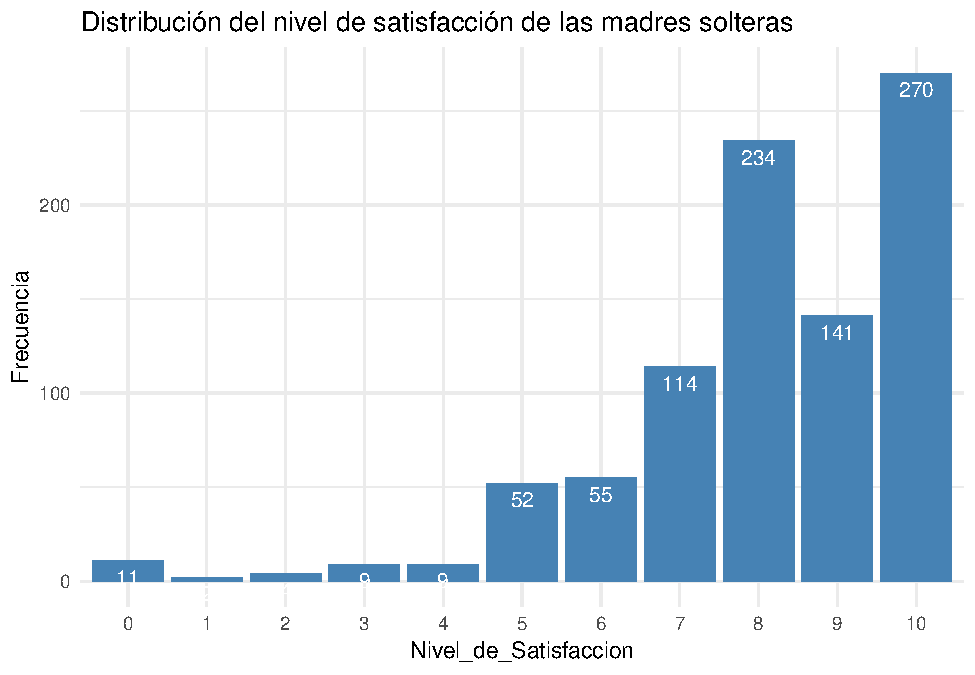
\includegraphics{barras2.pdf}
	\caption{Diagrama de barras, distribución de la satisfacción de las madres solteras}
\end{figure}



\vspace{100px}
\noindent
En la Figura 2 se muestra el diagrama de caja y bigotes de la distribución de la variable respuesta donde se puede observar que el un 75{\%} de las madres solteras tiene un nivel de satisfacción superior al nivel 7. 
\begin{figure}[H]
	\centering
	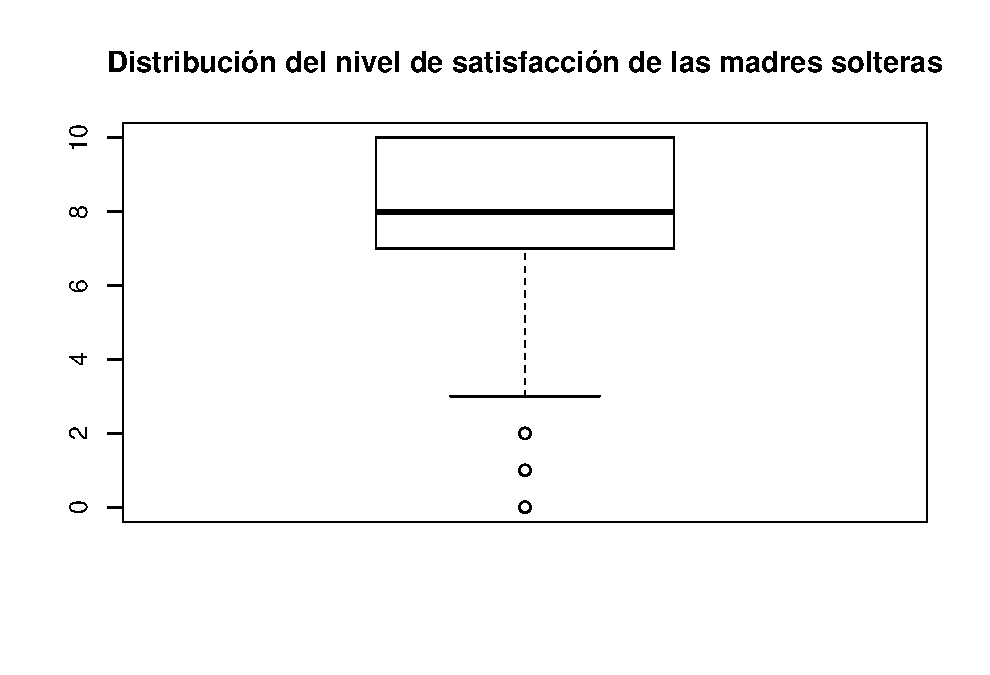
\includegraphics{boxplot1.pdf}
	\caption{Diagrama de caja y bigotes (boxplot) de la distribución de la satisfacción de las madres solteras}
\end{figure}
% hace falta porner otros graficoss****


\vspace{180px}
\noindent
En la Figura 3 se muestra un gráfico de barras de la distribución del número de hijos de las madres solteras, se puede observar que la existen 557 madres que tienen 1 solo hijo, mientras que apenas existen 7 mujeres con 5 hijos.  
\begin{figure}[H]
	\centering
	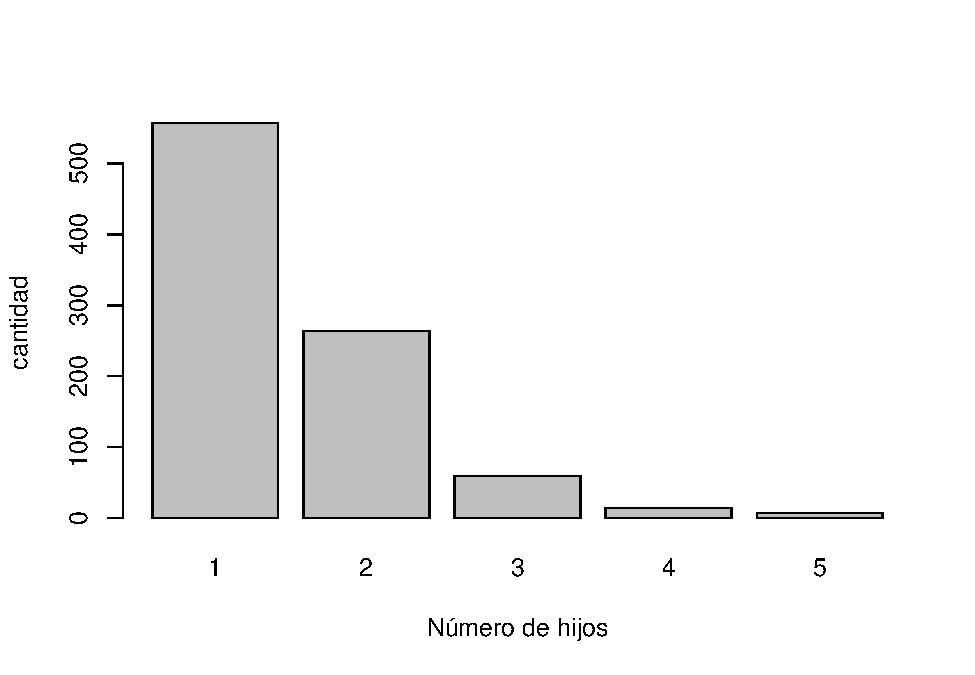
\includegraphics{barrasnumerodehijos.pdf}
	\caption{Distribución de la cantidad de hijos de las madres solteras}
\end{figure}

\vspace{180px}
\noindent
En la Figura 4 se muestra un gráfico de barras que muestra la distribución del número de nietos de la madre soltera, donde se observa que la mayoría de las madres solteras no tienen nietos aún.
\begin{figure}[H]
	\centering
	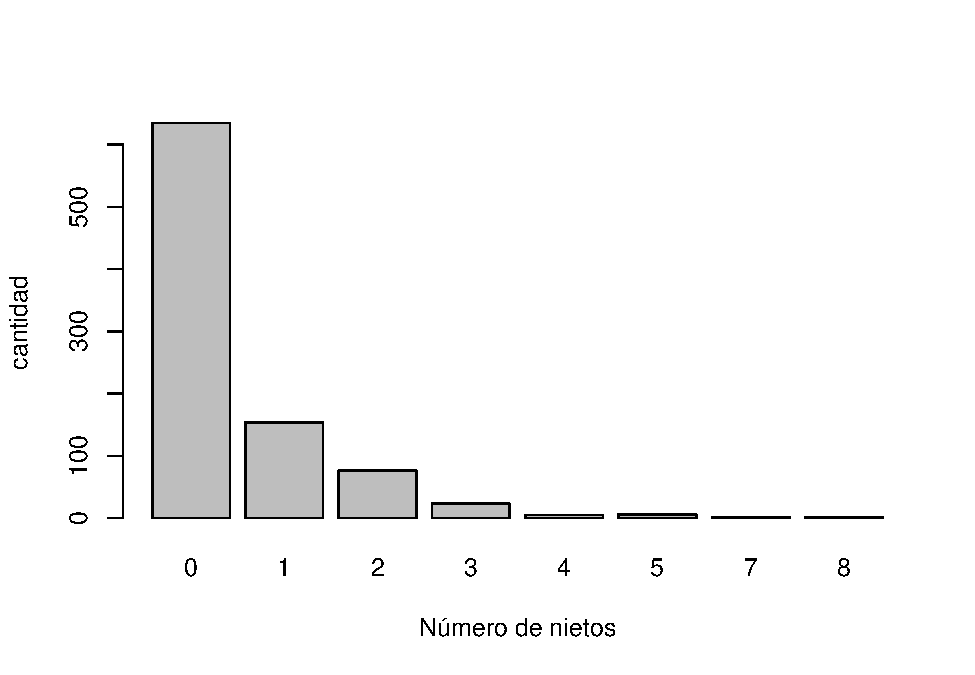
\includegraphics{barrasnumerodenietos1.pdf}
	\caption{Distribución de la cantidad de nietos de las madres solteras}
\end{figure}

\vspace{180px}
\noindent
En la Figura 5 se muestra la distribución del uso de las redes sociales donde ser puede observar que la mayor parte de las madres solteras no hacen uso de esta herramienta tecnológica.
\begin{figure}[H]
	\centering
	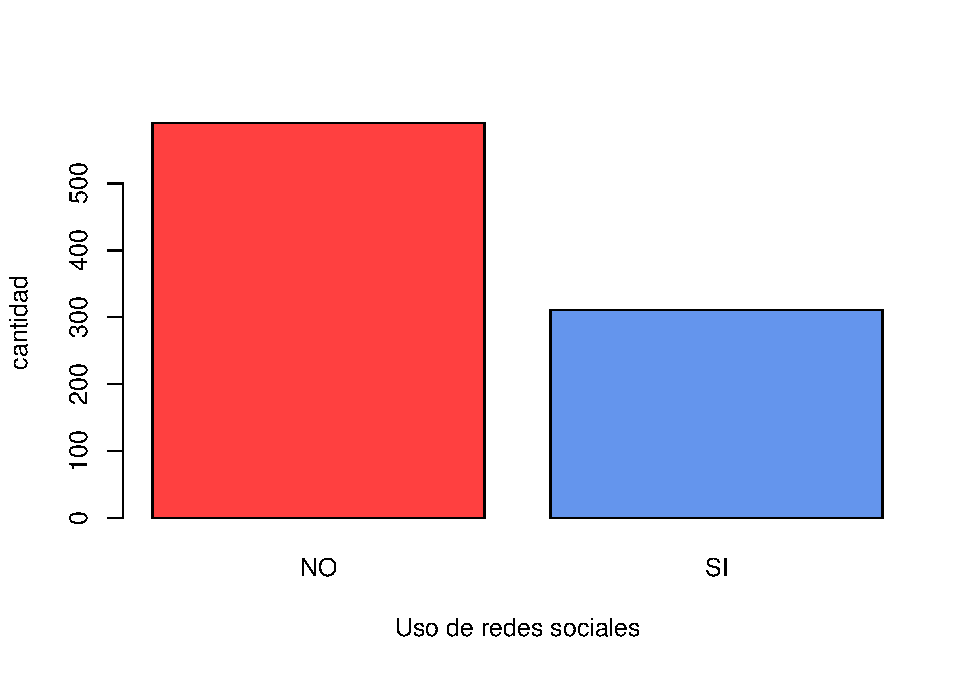
\includegraphics{usoderedes.pdf}
	\caption{Distribución del uso de la redes sociales}
\end{figure}



\subsection{Modelamiento estadístico}
\noindent
Se decidió implementar varios modelos de clasificación con el fin de comprar el rendimiento de cada modelo y seleccionar aquel que tuviera mayor tasa de clasificación de respuestas correctas, esto se hizo analizando la matriz de confusión.  
\\
\\
Antes de realizar el modelo de clasificación se realizó un modelo de regresión lineal múltiple haciendo uso de la funcion \texttt{lm()} (suponiendo inicialmente la variable respuesta como cuantitativa) esto con el fin de evaluar el proceso de selección de variables el cual se desarrolló haciendo uso función \texttt{stepGAIC()} de la librería MASS en el software estadístico R, lo cual permite usar un procedimiento de selección de variables hacia adelante (forward) y hacia atrás (backward), definiendo como frontera del modelo la combinación lineal de todas las variables explicativas categóricas (ya convertidas en variables dummy o factores) como también la interacción sencilla entre las variables explicativas cuantitativas.

\vspace{20px}
\noindent
En la Tabla 3 se muestra los estadísticos de resumen calculados con la función \texttt{lm()} del modelo de regresión lineal múltiple (suponiendo inicialmente variable respuesta como cuantitativa)

\begin{table}[H]
	\caption{\small{Resumen del modelo1}}
	\centering {\small
		\begin{tabular}{@{}cccc@{}}
			\toprule
			Modelo  & $R^{2}$  & $\rho_{y,\hat{y}}$  & AIC \\ \midrule
			Modelo1 & 0.47     & 0.71              & 3253.336\\ 
			\bottomrule
	\end{tabular}}
\end{table}


\noindent
Se hace un proceso de selección de variables haciendo uso de la función \texttt{stepGAIC()} con parámetro (\texttt{direction=’backward’}) para hacer selección hacia atrás, la variables seleccionadas se muestran en la Tabla 4.

\begin{table}[H]
	\caption{\small{Variables  seleccionadas}}
	\centering {\small
	\begin{tabular}{@{}rr@{}}
		\toprule
		Código de variable           &Variable  seleccionada                                  \\ \midrule
		P6040              & Edad  en años                               \\
		P1896              & Satisfacción con el ingreso                               \\
		P1897              & Satisfacción con la salud                  				 \\
		P1898              & Satisfacción con el nivel de seguridad                       \\
		P1901              & Nivel felicidad del día de ayer                                \\
		P1902              & Nivel de tranquilidad del día de ayer                           \\
		P1905              & Satisfacción con las cosas que hace                              \\
		P1084              & Frecuencia con la que usa internet                                \\
		P1083S3            & Uso de redes sociales                                              \\
		N\_HIJOS           & Número de hijos                                                     \\
		N\_NIETOS          & Número de nietos                                                     \\
		                                                  \\ \bottomrule
	\end{tabular}}
\end{table}



\noindent
En la Tabla 5 se muestra el resumen del modelo ajustado con las variable seleccionadas con la función \texttt{stepGAIC()}, se puede observar que la variables resultan considerablemente significativas en al menos uno de sus niveles, y que la estimación para el numero de hijos resulta ser negativa, por tanto se podría pensar que a mayor cantidad de hijos se vería afectado negativamente el nivel de satisfacción de las madres solteras, caso contrario se ve con el numero de nietos. 
\\
\\
Nota: se omite la estimación para algunos niveles de las variables dummy ya que al ser un nivel significativo para el modelo todos los demás niveles también lo serian.  

\begin{table}[H]
	\caption{\small{Resumen del modelo ajustado con la variables seleccionadas}}
	\centering
	\begin{tabular}{rrr}
		\hline
		& Estimación & Pr($>$$|$t$|$) \\ 
		\hline
		(Intercepto) & 1.2573 & 0.1578 \\ 
		P6040 & 0.0074 &  0.0340 \\ 
		P1896-1 & 1.7534 &  0.0008 \\ 
		P1896-2 & 0.9837 &  0.0112 \\ 
		. & . &  . \\ 
		
		P1897-1 & 1.4582 & 0.0179 \\ 
		P1897-2 & -0.1971 &  0.7670 \\ 
		P1897-3 & -0.5488 & 0.3097 \\ 
		. & . &  . \\ 
		P1898-1 & -1.7667 &  0.0147 \\ 
		P1898-2 & 0.0752 &  0.8951 \\ 
		P1898-3 & -0.5645 &  0.2563 \\ 
		. & . &  . \\ 
		P1901-1 & -0.0476 &  0.9529 \\ 
		P1901-2 & -1.6578 &  0.0208 \\ 
		P1901-3 & -1.0153 &  0.0694 \\ 
		. & . &  . \\ 
		P1902-1 & 2.7035 &  0.0002 \\ 
		P1902-2 & 2.0839 &  0.0004 \\ 
		P1902-3 & 0.3902 &  0.5179 \\ 
		. & . &  . \\ 
		P1905-1 & 4.9085 &  0.0025 \\ 
		P1905-2 & 2.0194 &  0.0836 \\ 
		P1905-3 & 3.7606 & 0.0005 \\ 
		. & . &  . \\ 
		N\_HIJOS & -0.0617 & 0.3495 \\ 
		N\_NIETOS & 0.0870 & 0.1101 \\ 
		P1084-2 & -0.1917 &  0.2905 \\ 
		P1084-3 & -0.0750 &  0.8450 \\ 
		P1084-5 & -0.1908 &  0.4284 \\ 
		P1083S3-1 & -0.0244 &  0.9164 \\ 
		\hline
	\end{tabular}
\end{table}




\noindent
\subsection*{Modelos de Clasificación}
 \noindent
Una vez seleccionadas las variables (ver Tabla 4) se procede a la implementación de varios modelos de clasificación con el fin de evaluar el rendimiento de cada uno y seleccionar aquel que tenga mayor tasa de clasificación correcta. 


\subsection*{Máquina de Soporte Vectorial con Kernel (Kernel SVM Classifier)}
\noindent
Las Máquinas de Soporte Vectorial son modelos capaces de generar clasificaciones o regresiones de datos no lineales a partir de la transformación de los datos de entrada a otros espacios de mayores dimensiones. En la Tabla 6 se puede observar que en la diagonal principal de la matriz están las predicciones correctas por cada nivel de satisfacción, donde se concluye que el modelo es deficiente para clasificar correctamente niveles de satisfacción de las madres solteras inferiores a 6, para el nivel 10 este modelo clasifico 208 observaciones bien y 62  mal, este ultimo fue el nivel donde mas aciertos obtuvo el modelo. 
\\
Para este modelo tenemos un total de 439 predicciones correctas, mientras que habrá un total de 462 predicciones incorrectas. Esto nos da una tasa clasificación correcta para el nivel de satisfacción del madres solteras de  0.48 es decir,  el 48\%.



% latex table generated in R 3.5.1 by xtable 1.8-3 package
% Wed Jan 30 14:51:59 2019
\begin{table}[H]
	\caption{\small{Matriz de confusión con SVM}}
	\centering
	\begin{tabular}{r|rrrrrrrrrrr}
		\hline
		& 0 & 1 & 2 & 3 & 4 & 5 & 6 & 7 & 8 & 9 & 10 \\ 
		\hline
		0 &   0 &   0 &   0 &   0 &   0 &   0 &   0 &   0 &   8 &   0 &   3 \\ 
		1 &   0 &   0 &   0 &   0 &   0 &   0 &   0 &   0 &   2 &   0 &   0 \\ 
		2 &   0 &   0 &   0 &   0 &   0 &   0 &   0 &   0 &   4 &   0 &   0 \\ 
		3 &   0 &   0 &   0 &   0 &   0 &   0 &   0 &   0 &   6 &   0 &   3 \\ 
		4 &   0 &   0 &   0 &   0 &   0 &   0 &   0 &   0 &   9 &   0 &   0 \\ 
		5 &   0 &   0 &   0 &   0 &   0 &   0 &   0 &   0 &  45 &   0 &   7 \\ 
		6 &   0 &   0 &   0 &   0 &   0 &   0 &   0 &   0 &  48 &   1 &   6 \\ 
		7 &   0 &   0 &   0 &   0 &   0 &   0 &   0 &   0 & 103 &   0 &  11 \\ 
		8 &   0 &   0 &   0 &   0 &   0 &   0 &   0 &   0 & 191 &   7 &  36 \\ 
		9 &   0 &   0 &   0 &   0 &   0 &   0 &   0 &   0 &  79 &  40 &  22 \\ 
		10 &   0 &   0 &   0 &   0 &   0 &   0 &   0 &   0 &  61 &   1 & 208 \\ 
		\hline
	\end{tabular}
\end{table}



\subsection*{Clasificador Bayesiano Ingenuo (Naive Bayes Classifier)}
\noindent
Este modelo es un clasificador fundamentalmente probabilístico y basado en el Teorema de Bayes. Se le dice ingenuo porque parte de la presunción de que todas las variables predictoras del modelo tienen total independencia lineal.
\\
Para este modelo tenemos un total de 491 predicciones correctas, mientras que habrá un total de 410 predicciones incorrectas. Esto nos da una tasa clasificación correcta para el nivel de satisfacción del madres solteras de 0.54 es decir,  el 54\%.

\begin{table}[H]
	\caption{\small{Matriz de confusión con Clasificador Bayesiano}}
	\centering
	\begin{tabular}{r|rrrrrrrrrrr}
		\hline
		& 0 & 1 & 2 & 3 & 4 & 5 & 6 & 7 & 8 & 9 & 10 \\ 
		\hline
		0 &   8 &   0 &   0 &   0 &   0 &   1 &   1 &   0 &   0 &   0 &   1 \\ 
		1 &   0 &   2 &   0 &   0 &   0 &   0 &   0 &   0 &   0 &   0 &   0 \\ 
		2 &   0 &   0 &   3 &   1 &   0 &   0 &   0 &   0 &   0 &   0 &   0 \\ 
		3 &   0 &   0 &   0 &   7 &   0 &   0 &   0 &   0 &   1 &   1 &   0 \\ 
		4 &   0 &   0 &   0 &   0 &   6 &   0 &   0 &   1 &   2 &   0 &   0 \\ 
		5 &   1 &   0 &   1 &   2 &   0 &  27 &   4 &   7 &   7 &   0 &   3 \\ 
		6 &   2 &   0 &   0 &   1 &   5 &   8 &  10 &   5 &  16 &   5 &   3 \\ 
		7 &   0 &   0 &   0 &   1 &   1 &   6 &  12 &  44 &  36 &   5 &   9 \\ 
		8 &   1 &   0 &   0 &   1 &   1 &   7 &  22 &  25 & 119 &  29 &  29 \\ 
		9 &   1 &   0 &   0 &   0 &   0 &   2 &   7 &   6 &  42 &  68 &  15 \\ 
		10 &   0 &   0 &   0 &   0 &   1 &   7 &   7 &   9 &  35 &  14 & 197 \\ 
		\hline
	\end{tabular}
\end{table}




\subsection*{Clasificación con Árbol de Decisión (Decision Tree Classifier)}
\noindent
Los Árboles de Decisión son modelos de predicción que pueden usarse tanto para clasificación como para regresión, y cuyo funcionamiento se basa en la construcción de reglas lógicas (divisiones de los datos entre rangos o condiciones) a partir de los datos de entrada.
\\
Para este modelo tenemos un total de 463 predicciones correctas, mientras que habrá un total de 438 predicciones incorrectas. Esto nos da una tasa clasificación correcta para el nivel de satisfacción del madres solteras de 0.51 es decir,  el 51\%.
\begin{table}[H]
	\caption{\small{Matriz de confusión con Árbol de Decisión}}
	\centering
	\begin{tabular}{r|rrrrrrrrrrr}
		\hline
		& 0 & 1 & 2 & 3 & 4 & 5 & 6 & 7 & 8 & 9 & 10 \\ 
		\hline
		0 &   0 &   0 &   0 &   0 &   0 &   9 &   0 &   0 &   0 &   0 &   2 \\ 
		1 &   0 &   0 &   0 &   0 &   0 &   1 &   0 &   0 &   1 &   0 &   0 \\ 
		2 &   0 &   0 &   0 &   0 &   0 &   4 &   0 &   0 &   0 &   0 &   0 \\ 
		3 &   0 &   0 &   0 &   0 &   0 &   7 &   0 &   0 &   1 &   0 &   1 \\ 
		4 &   0 &   0 &   0 &   0 &   0 &   3 &   0 &   4 &   2 &   0 &   0 \\ 
		5 &   0 &   0 &   0 &   0 &   0 &  25 &   0 &   8 &  12 &   0 &   7 \\ 
		6 &   0 &   0 &   0 &   0 &   0 &  17 &   0 &   8 &  27 &   0 &   3 \\ 
		7 &   0 &   0 &   0 &   0 &   0 &  15 &   0 &  28 &  58 &   2 &  11 \\ 
		8 &   0 &   0 &   0 &   0 &   0 &  16 &   0 &  14 & 154 &  19 &  31 \\ 
		9 &   0 &   0 &   0 &   0 &   0 &   5 &   0 &   5 &  51 &  61 &  19 \\ 
		10 &   0 &   0 &   0 &   0 &   0 &  14 &   0 &   5 &  48 &   8 & 195 \\ 
		\hline
	\end{tabular}
\end{table}



\subsection*{Clasificador con Bosques Aleatorios (Random Forests Classifier)}
\noindent
La clasificación con Bosques Aleatorios o Random Forests, implica la construcción al azar de una gran cantidad de árboles de decisión sobre un mismo conjunto de datos, y la decisión final de la clasificación es tomada a partir de calcular el voto de la mayoría de las predicciones ofrecidas por cada uno de los árboles que conforman el bosque.
\\
Para este modelo tenemos un total de 898 predicciones correctas, mientras que habrá un total de 3 predicciones incorrectas. Esto nos da una tasa clasificación correcta para el nivel de satisfacción del madres solteras de  0.99 es decir,  el 99\%.

\begin{table}[H]
	\caption{\small{Matriz de confusión con Bosques Aleatorios}}
	\centering
	\begin{tabular}{r|rrrrrrrrrrr}
		\hline
		& 0 & 1 & 2 & 3 & 4 & 5 & 6 & 7 & 8 & 9 & 10 \\ 
		\hline
		0 &  11 &   0 &   0 &   0 &   0 &   0 &   0 &   0 &   0 &   0 &   0 \\ 
		1 &   0 &   2 &   0 &   0 &   0 &   0 &   0 &   0 &   0 &   0 &   0 \\ 
		2 &   0 &   0 &   4 &   0 &   0 &   0 &   0 &   0 &   0 &   0 &   0 \\ 
		3 &   0 &   0 &   0 &   9 &   0 &   0 &   0 &   0 &   0 &   0 &   0 \\ 
		4 &   0 &   0 &   0 &   0 &   9 &   0 &   0 &   0 &   0 &   0 &   0 \\ 
		5 &   0 &   0 &   0 &   0 &   0 &  52 &   0 &   0 &   0 &   0 &   0 \\ 
		6 &   0 &   0 &   0 &   0 &   0 &   0 &  55 &   0 &   0 &   0 &   0 \\ 
		7 &   0 &   0 &   0 &   0 &   0 &   0 &   0 & 114 &   0 &   0 &   0 \\ 
		8 &   0 &   0 &   0 &   0 &   0 &   0 &   0 &   0 & 232 &   1 &   1 \\ 
		9 &   0 &   0 &   0 &   0 &   0 &   0 &   0 &   0 &   0 & 141 &   0 \\ 
		10 &   0 &   0 &   0 &   0 &   0 &   0 &   0 &   0 &   0 &   0 & 270 \\ 
		\hline
	\end{tabular}
\end{table}





\subsection{Diagnóstico del Modelo}

A continuación se muestra una tabla de resumen de los modelos de clasificación implementados. 

\begin{table}[H]
		\caption{\small{Resumen de modelos de clasificación}}
	\centering
	\begin{tabular}{@{}cc@{}}
		\toprule
		Modelo                         & Clasificación Correctas \\ \midrule
		SVM                            & 48\%                    \\
		Clasificador Bayesiano Ingenuo & 54\%                    \\
		Árbol de Decisión              & 51\%                    \\
		Bosques Aleatorios             & 99\%                    \\ \bottomrule
	\end{tabular}
\end{table}

\noindent
El clasificador con Bosques Aleatorios es el modelo que mejor resultado ofrece en la clasificación de del nivel de satisfacción de las madres solteras. 



%***-----------------------------------------CONCLUCIONES--------------------------------------------------
\section{Conclusiones}


Para el moldeamiento estadístico que involucra una variable respuesta de tipo categórico ordinal en el caso en que esta tenga más de dos categorías, es preciso y más eficiente utilizar eu modelo de clasificación, en este caso particular el modelo que mejor presento rendimiento del modelo de bosques aleatorios. El planteado funciona correctamente para predecir la satisfacción de las mujeres solteras en función de las características y composición del hogar como número de hijos y número de nietos, niveles subjetivos de satisfacción en seguridad, salud, felicidad y tranquilidad como también variables de acceso a tecnologías de la información y comunicación como acceso a internet y a redes sociales, es por esto que este fue el modelo que se implementó en la aplicación web \textbf{StatiSfoft 2.0}





%***----------------------------------------APLICACION WEB--------------------------------------------
\section{Aplicación web}






%***----------------------------------------REFERENCIAS--------------------------------------------
\section{Referencias}
[1] El estudio de la satisfacción con la vida, Ruut Veenhoven 

[2] Problemas que debe enfrentar una madre soltera - https://madresoltera.org/problemas/

[3] Modelos de clasificación con R -https://rpubs.com/rdelgado/397838

[4] RStudio Team: (2018). Integrated Development for R. RStudio, Inc., Boston, MA URL
http://www.rstudio.com/.



\end{document}